\documentclass[a4paper, 11pt]{article}
\usepackage{geometry}
\usepackage{indentfirst}
\usepackage{setspace}
\usepackage{amsmath}
\usepackage{amssymb}
\usepackage{graphicx}
\usepackage{wrapfig}
\usepackage{caption}
\usepackage{indentfirst}
\setlength{\parindent}{20pt}
\usepackage{amssymb}
\usepackage{float}
\usepackage{subcaption}

\usepackage[backend=biber,style=ieee, sorting=none, sortlocale=en_US]{biblatex}
\bibliography{biblio.bib}

\graphicspath{ {./images/} }
\geometry{left=2.5cm, right=2.5cm, top=2.5cm, bottom=2.5cm}

\begin{document}	
	\title{Essay - Cognition and Computation }
	\author{{\small Alexandre da Rocha Rodrigues (2039952)}}
	\date{\today}
	\maketitle
	
	\section{Introduction}
	
		The EMNIST  Balanced dataset is derived from the NIST Special Database 19 \cite{emnist}\cite{ExpEMNIST}.
		It has 47 classes: digits (0-9), uppercase letters (A-Z) and some lowercase letters (a,b,d,e,f,g,h,n,q,r,t).
		It consists in a total of 131600 samples, 112800 being for training and 18800 for testing.
		It provides a consistent and fair classification, with equal number of samples for each class, despite being sufficiently challenging. 
		
		A possible neural network used to model and classify these samples is the Deep Belief Network.
		It consists in a composition of Restricted Boltzmann Machines, the hidden layer of one serves as visible layer of the next.
		
		A RBM is generative stochastic neural network used to learn the probability distribution over its inputs.
		This implies that the activation level of a neuron is a representation of a probability.
		The input is present in a set of visible neurons.
		It can extract statistical structure information in a set of hidden neurons.
		We use maximum likelihood learning to update the weights aiming for a accurate top-down reconstruction.
		The most probable configurations of hidden and visible neurons are specified by the energy function based on the connection weights.
		
		These characteristics of RBMs allows us to use a stack of them, a DBN, to learn multiple levels of representation and thus better hidden representations that can serve as examples of a class.
		The DBN is trained with the constrastive divergence algorithm, reducing the discrepancy between the real and the learned probability distribution.
		
		A Perceptorn is a simple neural network model with a set of inputs and a single binary output.
		We can hereby use a set of 47 Perceptrons, one corresponding to each class, to classify the samples, using the final hidden layer of the DBN as their inputs.
		
		Feedforward Neural Networks are multiple layers of Perceptrons, having one or more hidden layers.
		In this case, we use the Rectified Linear Unit activation function to avoid the weakening of the error gradient.
		
	
	\section{Hyper Parameters}
		The parameters used can be found in the following table.
		\begin{table}[H]
			\centering
			\begin{tabular}{c|c}
				\textbf{Parameter} 		& \textbf{Value} 	\\ \hline
				Hidden Layers Sizes 	& $ 1000,1000 $    	\\ \hline
				Gibbs Sampling Steps (k)&  $ 1 $      		\\ \hline
				Learning Rate			&  $ 0.1 $     		\\ \hline
				Initial Momentum		&  $ 0.9 $    		\\ \hline
				Final Momentum			&  $ 0.9 $    		\\ \hline
				Weight Decay			&  $ 0.00001 $      \\
			\end{tabular}
			\caption{Hyper Parameters of the Deep Belief Network}
			\label{tab:pars}
		\end{table}
		
		These parameters were isolated and tested.
		Starting from the parameters of the first lab notebook, I changed only one of the parameters and found the best value.
		Repeated this for all parameters and used the best of each.
		This does not guarantee the best results because the parameters can be the best when isolated but not the best combination of all of them.
		We can although consider these values as a good approximation to the best case.
		The objective was to reduce the average reconstruction error in the DBN training phase.
		
		Enabling learning rate decay decreased the average reconstruction error but the weight representations were not as expected, due to a very small gradient, so it will be disabled in this case.	
		The Xavier weights initialization is also disabled because it did not produce any measurable performance improvement.
		
		To serve as comparison we can use Feedforward Neural Networks, one with 1 hidden layer and another with 2 hidden layers, all of size $ 1000 $.
		
		The Perceptron and FFNNs were trained in the same way, using an stochastic gradient descent optimizer with learning rate of $ 0.05 $ and the cross entropy loss function, for $ 1000 $ epochs. 
				
		
	\section{Results}
		To achieve a training time close to the sum of the DBN and Perceptron training time, the FFNN with 2 hidden layers was trained in 60 epochs and the one with 1 hidden layer was trained in 150 epochs.
		
			\begin{table}[H]
				\centering
				\begin{tabular}{c|c}
					DBN 					&  $ 474 s $    \\ \hline
					Perceptron 				&  $ 453 s $      \\ \hline
					FFNN with 1 layer		&  $ 932 s $     \\ \hline
					FFNN with 2 layers		&  $ 927 s $    \\
				\end{tabular}
				\caption{Training Time}
				\label{tab:Ttime}
			\end{table}
			
		\subsection{Accuracy}
			\begin{table}[H]
				\centering
				\begin{tabular}{c|c}
					DBN 					&  $ 61.95\% $    \\ \hline
					FFNN with 1 layer		&  $ 30.76\% $     \\ \hline
					FFNN with 2 layers		&  $ 14.37\% $    \\
				\end{tabular}
				\caption{Accuracy}
				\label{tab:acc}
			\end{table}
			The DBN accuracy is a very good result, given that the EMNIST article \cite{emnist} shows a $ 64\% $ result for a OPIUM-based model with hidden layer size of $ 1000 $.
			The FFNNs produce lower accuracy as expected, the addition of a second hidden layer significantly decreased accuracy.
			
	
		\subsection{Representations}
			\begin{figure}[H]
				\begin{subfigure}{.49\textwidth}
					\centering
					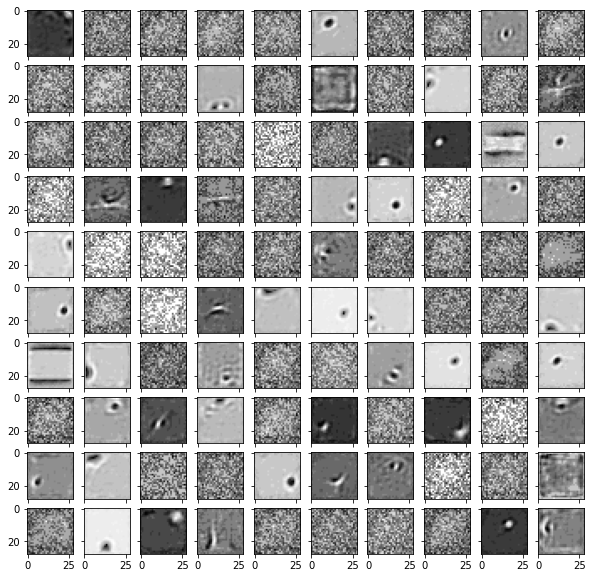
\includegraphics[width=.99\linewidth]{0.1_1.png}  
					\caption{Representation of the 1st hidden layer}
					\label{fig:rep1}
				\end{subfigure}
				\begin{subfigure}{.49\textwidth}
					\centering
					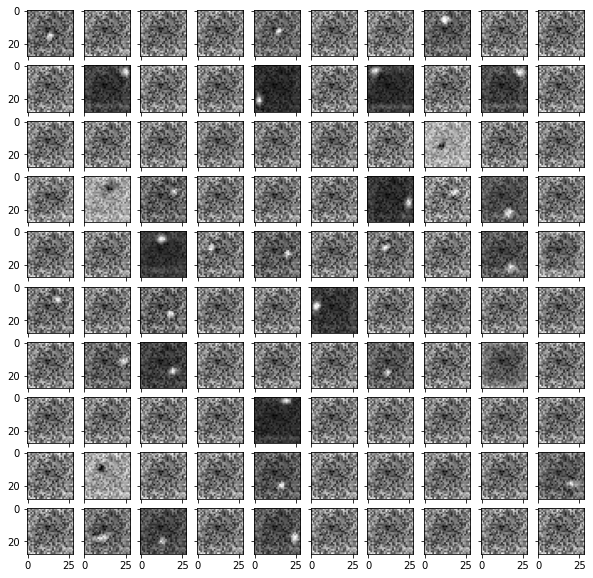
\includegraphics[width=.99\linewidth]{0.1_2.png}  
					\caption{Representation of the 2nd hidden layer}
					\label{fig:rep2}
				\end{subfigure}
				\caption{Representations of the DBN hidden layers}
				\label{fig:rep}
			\end{figure}
			These results can be interpreted as the parts of the images that make each neuron of the hidden layer activate.
			The first hidden layer shows some dot like features, meaning that the neurons focus on small regions of the image.
			The 2nd hidden layer representation is more noisy, we can conclude that it does not develop very useful features.
		
		\subsection{Dendrograms}
		
			\begin{figure}[H]
				\centering
				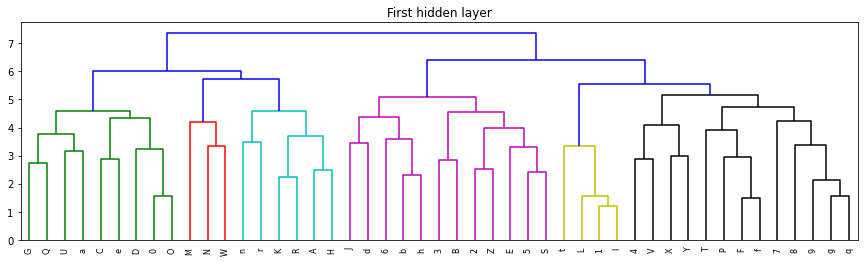
\includegraphics[width=.8\linewidth]{dend1.png}  
				\caption{Dendrogram for first hidden layer}
				\label{fig:dend1}
			\end{figure}
		
			\begin{figure}[H]
				\centering
				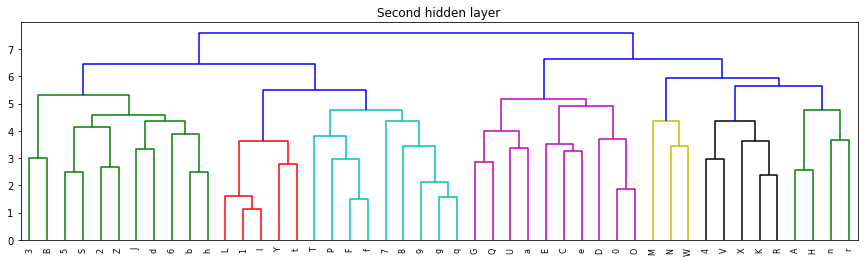
\includegraphics[width=.8\linewidth]{dend2.png}  
				\caption{Dendrogram for second hidden layer}
				\label{fig:dend2}
			\end{figure}
		
			 These figures shows that the both hidden representation evaluates "l" and "1" as the most similar symbols, "L" is the next most similar to both \cite{Dends}.
			 Other similar symbols are: "F" and "f", "g" and "q".
			 The easiest distinctions for the model to make are represented as the first branching when reading from top to bottom.
			 
			 The second hidden representation shows more uniform branching.
			 As an example, we can see "n" and "r" are at an height of $ 3 $ in the first hidden representation, but $ 4 $ on the second.
			 These dendrograms are, although, almost equivalent.
			 
		\subsection{Confusion Matrix}	
			\begin{figure}[H]
				\centering
				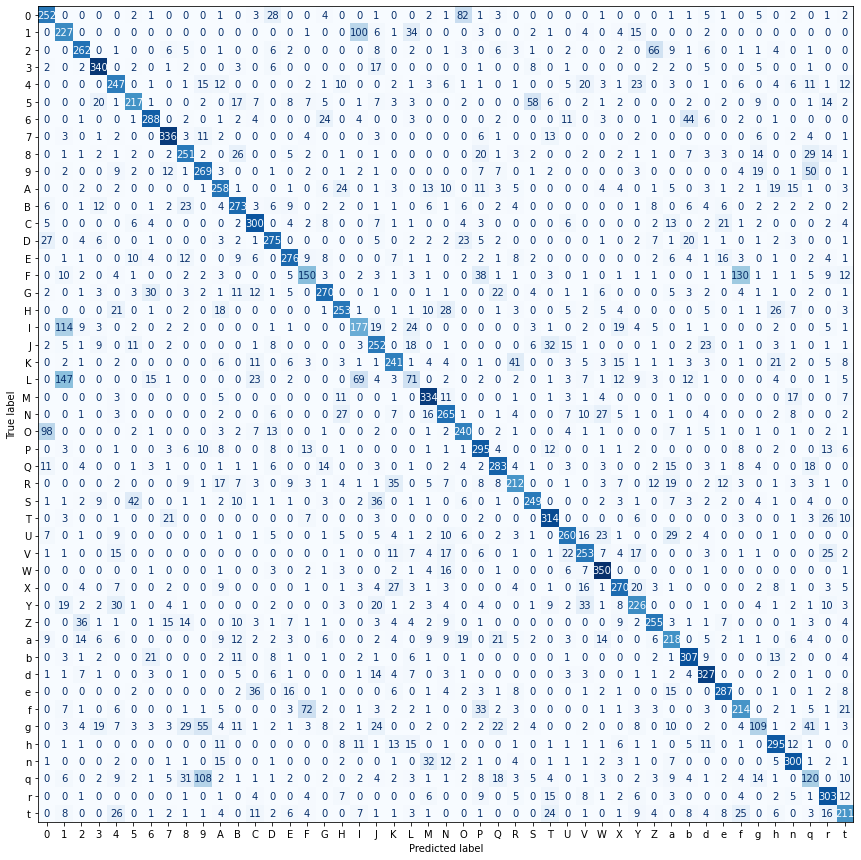
\includegraphics[width=.9\linewidth]{confmatBlue2.png}
				\caption{Confusion Matrix}
				\label{fig:confmat}
			\end{figure}
		
			The confusion matrix shows the correspondence between the predicted label and the true label.
			This allows us to check model errors and thus what confuses the model.
			The ideal confusion matrix would have only non zeros in the diagonal.
			
			The highest values outside the diagonal are the most similar symbols found by the model.
			These results are equivalent to the dendograms, largest values in the confusion matrix correspond to lower clades in the dendograms.

			The largest values are for: "L" labeled as "1", "F" labeled as "f", "I" as "1" and "q" as "9".
			 
			
		\subsection{Robustness to Noise}	
			\begin{figure}[H]
				\centering
				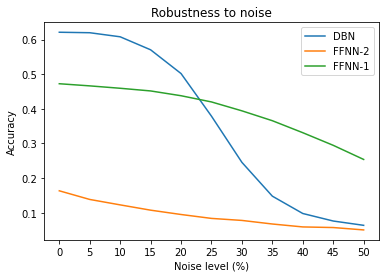
\includegraphics[width=.5\linewidth]{noise3.png} 
				\caption{Robustness to noise}
				\label{fig:robNoise}
			\end{figure}
		
			The DBN is clearly superior for small levels of noise.
			We can although see that the FFNN with 1 hidden layer is better for noise levels over $ 25\% $.\\
			We can also conclude that FFNNs are less affected by noise.
		
	\section{Conclusion}
		We can conclude that a Deep Belief Network comibined with a Perceptron layer is a good approach to classify letters and digits.
		Feedforward neural networks are a simpler and thus less effective model but can be very robust to noise. 
			
	%% BIBLIOGRAPHY	
	\printbibliography
				
\end{document}



